\scanpage{15}
% archive sheet number: 14
\uline{et transversal}.

e) \unsure{\deleted{c}C|\deleted{C}c|\deleted{o}C|\deleted{C}o}ompatibilité avec \uline{changement de base} $S'\handwritten{\longrightarrow}S$, avec \uline{produits cartésiens} $Y_1\mathbin{\mathrm{x}}_S Y_2$ sur $S$.

\unsure{\deleted{f}g|\deleted{g}f}) Indépendance par rapport à $S$. \handwritten{($S\unsure{\neg|\text{---}|\longrightarrow}T$)}
\margin{\handwritten{\figure{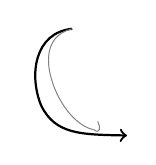
\begin{tikzpicture}[x=.012cm,y=-.012cm]
\draw[line width=.8pt,->] (48,27) .. controls (8,31) and (2,76) .. (15,108) .. controls (30,139) and (57,139) .. (106,140);
\draw[gray,line width=.35pt] (48,27) .. controls (15,35) and (20,71) .. (32,96) .. controls (42,117) and (57,131) .. (71,134) .. controls (78,139) and (78,131) .. (75,125);
\end{tikzpicture}}}}

f) Compatibilité avec changement d'anneau.

h) Re\unsure{\deleted{m}l|\deleted{l}m}ation avec Gysin: Les classes (4.8),(4.9) s'interprètent comme l'image de $1_X$ par Gysin. Le transformé de (4.4) par $\mathrm{R}f_{\handwritten{!}}$, suivi de l'homomorphisme d'adjonction, est l'homomorphisme de Gysin.

Je pense que, compte tenu du formulaire d\unsure{\deleted{u}e|\deleted{e}u|\deleted{a}u|\deleted{u}a} par.4, le formulaire \deleted{ici} proposé ici pour les classes fondamentales $\pm$ locales est pratiquement trivial\deleted{\unsure{,|e|.}} à partir des définitions. On peut \deleted{don}, pour finir, récupérer un énoncé qui donne la \uline{caractérisation} des classes fondamentales locales dans le cas d'un couple lisse, par les propriétés suivantes 1) Nature locale (pour Zar suffit) 2) cas $p=0$ 3) cas $p=1$, quand $X$ est défini par une équation 4) propriété de cup-produit d) (où il suffit de pre\unsure{\deleted{d}n|\deleted{n}d}\unsure{\deleted{n}d|\deleted{d}n}re un des deux facteurs de codimension 1). Signaler\inserted{en remarque} que cet énoncé\deleted{\unsure{,|(}}\inserted{(existence et unicité d'une théorie des cl. fond. loc.)} peut se démontrer sans difficulté indépendamment de la théorie de dualité et de celle de l'homomorphisme trace, et avait été donnée dans le séminaire oral \deleted{\unsure{au|en} prélimi} avant la dualité.

Remords: il serait pr\unsure{\deleted{i}u|\deleted{u}i}\unsure{d|\deleted{u}d|\deleted{d}u|\deleted{a}d|\deleted{d}a}ent d'adjoindre au formulaire un
\margin{\handwritten{\figure{\begin{tikzpicture}[x=.005cm,y=-.005cm]
\draw[line width=.4pt,->] (195,891) .. controls (90,730) and (12,565) .. (14,402) .. controls (12,216) and (88,99) .. (256,34);
\draw[line width=.35pt] (291,843) .. controls (265,860) and (217,896) .. (197,897) .. controls (172,912) and (139,1005) .. (131,1110) .. controls (124,1250) and (111,1389) .. (114,1437) .. controls (116,1464) and (134,1476) .. (147,1475);
\draw[line width=.4pt] (196,889)--(234,888);
\end{tikzpicture}}}}

i) On a commutativité dans le diagramme suivant
\diagram{\begin{tikzcd}[ampersand replacement=\&,column sep=3em,row sep=2em]
f^*(G)(\inserted{\handwritten{\unsure{-|=}}}p)\handwritten{[}\inserted{\handwritten{-}}2\unsure{\deleted{p}\handwritten{\delta}|\handwritten{p}|\deleted{)}\handwritten{p}}\handwritten{]} \handwritten{\arrow[r]} \handwritten{\arrow[dr,bend right=18]} \& \mathrm{R}f^{\handwritten{!}}(G) \\
\& \mathrm{R}f^{\handwritten{!}}(A_Y)\overset{\underline{\mathrm{L}}}{\otimes}{\unsure{\deleted{g}\handwritten{f}|\deleted{f}g}}^{\handwritten{*}}(G) \handwritten{\arrow[u]}
\end{tikzcd}},
où la flèche horizontale est (4.4), la flèche oblique est déduite par $\overset{\underline{\mathrm{L}}}{\otimes}G$ de (4.\unsure{\deleted{9}5|\deleted{5}9|\deleted{4}5|\deleted{5}4}),\deleted{dans le cas} et le flèche verticale est l'homomorphisme canonique qu'on devine,\deleted{(et} analogue à celui de changement de base pour les \handwritten{\textsuperscript{$!$}}, et qui manque dans 3.1\handwritten{(}tout comme ce dernier\handwritten{)}. On s'y intéressera sans doute surtout si $G$ est localement libre, donc l'homomorphi\unsure{s}me en question est un isomorphisme.
